\documentclass{exam}
\usepackage{amsmath,enumerate,tikz,xcolor}
\usepackage{graphicx}
 \graphicspath{{../Images/}}
\usepackage{float}
\pagestyle{empty}
\textwidth16cm
\textheight23cm
\oddsidemargin0pt
\topmargin-50pt
\def\R{\rule[-1ex]{0ex}{3.5ex}}
\def\ans#1{\hfill \textcolor{lightgray}{#1}}

\begin{document}
\noindent
Tougaloo College\hfill  {\small Final Exam Time: 9:00 - 11:00 am}\\
Spring 2020 \hfill {\small Final Exam Date: Monday, Apr. 27}\\ 
\begin{center}
{\bf MATH 221 Cal I Final Exam Review and Practice} 
\end{center}

\medskip
\noindent
%Name:\underline{\hspace{3in}} \hfill Score:\underline{\hspace{0.8in}}

\medskip
\begin{enumerate}
\item
Find the value of the limit, and, when applicable, indicate the limit theorems being used.  %\ans{(sec. 0.8 \#15)}


\begin{minipage}{.5\linewidth}
\begin{align*}
 f^{\prime}(0)&= \lim_{x\to0} \frac{\sqrt{x+2}-\sqrt{2}}{x}\\
&= \lim_{x\to0} \frac{\sqrt{x+2}-\sqrt{2}}{x}\cdot \frac{\sqrt{x+2}+\sqrt{2}}{\sqrt{x+2}+\sqrt{2}}\\
\end{align*}
\end{minipage}%
\begin{minipage}{.5\linewidth}
\begin{align*}
f^{\prime}(0)&=  \lim_{x\to0} \frac{1-\cos{x}}{\sin{x}}\\
 &=\lim_{x\to0} \frac{1-\cos{x}}{\sin{x}}\cdot \frac{x}{x}\\
&=\lim_{x\to0} \frac{1-\cos{x}}{x}\cdot \frac{x}{\sin{x}}\\
\end{align*}
\end{minipage}
\vfill

\begin{minipage}{.5\linewidth}
\begin{align*}
 f^{\prime}(2)&=\lim_{x\to 2} \frac{\frac{1}{x}-\frac{1}{2}}{x-2}\\
&=\lim_{x\to 2} \frac{\frac{2}{2x}-\frac{x}{2x}}{x-2} \\
&=\lim_{x\to 2} \frac{\frac{2-x}{2x}}{x-2} \\
\end{align*}
\end{minipage}%
\begin{minipage}{.5\linewidth}
\begin{align*}
 f^{\prime}(2^{-})&=\lim_{x\to 2^{-}} \frac{x^{3}+8}{x^{2}-4}\\
&=\lim_{x\to 2^{-}} \frac{(x+2)(x^{2}-2x+4)}{(x+2)(x-2)}\\
&=\lim_{x\to 2^{-}} \frac{x^{2}-2x+4}{x-2}\\
&=\frac{(2^{-})^{2}-2(2^{-})+4}{(2^{-})-2}\\
&=\frac{4}{0^{-}}=-\infty
\end{align*}
\end{minipage}



\item
Let 
\begin{align*}
f(x)=\frac{x^{2}-9}{|x-3|}=\frac{(x+3)(x-3)}{|x-3|}=(x+3)\frac{x-3}{|x-3|}
\end{align*}

Find each limit (if it exists).

\begin{minipage}{.3\linewidth}
\begin{align*}
 &\lim_{x\to 3^{-}}f(x)\\
 &=\lim_{x\to 3^{-}}(x+3)\frac{x-3}{|x-3|}\\
 &=\lim_{x\to 3^{-}}(x+3)\cdot\lim_{x\to 3^{-}}\frac{x-3}{|x-3|}\\
 &=(3+3)\cdot (-1) = -6
\end{align*}
\end{minipage}%
\begin{minipage}{.5\linewidth}
\begin{align*}
 &\lim_{x\to 3^{+}}f(x)\\
 &=\lim_{x\to 3^{+}}(x+3)\frac{x-3}{|x-3|}\\
 &=\lim_{x\to 3^{+}}(x+3)\cdot\lim_{x\to 3^{+}}\frac{x-3}{|x-3|}\\
 &=(3+3)\cdot (1) = -6
\end{align*}
\end{minipage}%
\begin{minipage}{.2\linewidth}
\begin{equation*}
 \lim_{x\to 3}f(x) = DNE
\end{equation*}
\end{minipage}

\vfill


%%%%%%%%%%%%%%%%%%%%%%%%%%%%%%%%%%%%%%%%%%%%%%%%%%%%%%%%-----New Page-----%%%%%%%%%%%%%%%%%%%%%%%%%%%%%%%%%%%%%%%%%%%
\newpage

\item
Let 
\[   f(x)=\left\{
\begin{array}{ll}
      x+2, & x\leq -1 \\
      x^{2}-1,& -1\leq x < 2\\
      \sqrt{x+1},   & x>2 \\
\end{array} 
\right. \]

Find each limit (if it exists).

\begin{minipage}{.3\linewidth}
\begin{align*}
 &\lim_{x\to -1^{-}}f(x)\\
 &=(-1)+2=1
\end{align*}
\end{minipage}%
\begin{minipage}{.3\linewidth}
\begin{align*}
 &\lim_{x\to -1^{+}}f(x)\\
 &=(-1)^{2}-1=0
\end{align*}
\end{minipage}%
\begin{minipage}{.3\linewidth}
\begin{align*}
 \lim_{x\to -1}f(x)=\text{DNE}
\end{align*}
\end{minipage}

\vfill


\begin{minipage}{.3\linewidth}
\begin{align*}
 &\lim_{x\to 2^{-}}f(x)\\
 &=(2)^{2}-1=3
\end{align*}
\end{minipage}%
\begin{minipage}{.2\linewidth}
\begin{align*}
 &\lim_{x\to 2^{+}}f(x)\\
 &=\sqrt{2+1}\\
 &=\sqrt{3}
\end{align*}
\end{minipage}%
\begin{minipage}{.2\linewidth}
\begin{align*}
 &\lim_{x\to 2}f(x)\\
 &=\text{DNE}
\end{align*}
\end{minipage}
\begin{minipage}{.2\linewidth}
\begin{align*}
 &\lim_{x\to 3}f(x)
 &=\sqrt{3}
\end{align*}
\end{minipage}
\vfill

\item Suppose that $$\lim_{x\to 3}(4f(x)-5g(x))=1$$ and $\lim_{x\to 3}2g(x)=6$. Find the value of $\lim_{x\to 3}f(x)$
\vfill\vfill


\item Suppose that 
\[   f(x)=\left\{
\begin{array}{ll}
     \frac{(x+5)^{2}-25}{2x}, & x \neq 0 \\
      c,   & x=0 \\
\end{array} 
\right. \]
If $f(x)$ is continuous at all real numbers, what is the value of $c$? \\
When $x \neq 0$, $f(x)$ is $\frac{0}{0}$ Form. There exist common factor between Numerator and Denominator. So the first step is to cancel common factor
\begin{align*}
 f(x)  & = \frac{(x+5)^{2}-25}{2x}\\
       & = \frac{(x)^{2}+10x+25-25}{2x} \\   
       & = \frac{(x)^{2}+10x}{2x} \\
       & = \frac{x+10}{2} \\
\end{align*}
Step 2: Set $f(x)=c$ at $x=0$, that is $\frac{x+10}{2}=c$ at $x=0$. Then we have $c=5$

%\item
%Find the limit L. Then use the $\varepsilon-\delta$ definition to prove that the limit is L.
%\[ 
%\lim_{x\to 2} (3x+2)
%\]
%\vfill



%%%%%%%%%%%%%%%%%%%%%%%%%%%%%%%%%%%%%%%%%%%%%%%%%%%%%%%%-----New Page-----%%%%%%%%%%%%%%%%%%%%%%%%%%%%%%%%%%%%%%%%%%%
\newpage

\item Find the following derivatives.

\begin{parts}
\part $f(x)=2x^{5}+\frac{1}{\sqrt[3]{x^{2}}}-\pi$
\vfill
\part  $h(x)=\frac{2x^{3}+4}{x^{2}-4x+1}$
\vfill
\end{parts}


\item Let $g(x)=\frac{1}{x^{2}}$, use the $\bf{Limit Definition}$ of the Derivative to find $g^{\prime}(x)$

\begin{align*}
f^{\prime}(x) & = \lim_{h\rightarrow 0}\frac{f(x+h)-f(x)}{h}\\
      & = \lim_{h\rightarrow 0}\frac{\frac{1}{(x+h)^{2}}-\frac{1}{x^{2}}}{h}\\
      & = \lim_{h\rightarrow 0}\frac{\frac{x^{2}}{x^{2}(x+h)^{2}}-\frac{(x+h)^{2}}{x^{2}(x+h)^{2}}}{h}\\
      & = \lim_{h\rightarrow 0}\frac{\frac{x^{2}-(x^{2}+2hx+h^{2})}{x^{2}(x+h)^{2}}}{h}\\
      & = \lim_{h\rightarrow 0}\frac{\frac{-2hx-h^{2}}{x^{2}(x+h)^{2}}}{h}\\
      & = \lim_{h\rightarrow 0}\frac{-h(2x+h)}{x^{2}(x+h)^{2}}\cdot \frac{1}{h}\\
      & = \lim_{h\rightarrow 0}\frac{-(2x+h)}{x^{2}(x+h)^{2}}\\
      & = \frac{-(2x+0)}{x^{2}(x+0)^{2}}\\
      & = -\frac{2}{x^{3}}\\
\end{align*}

\newpage

\item
Let
\[ 
f(x)=2\cos{x}-(\sqrt{2})x
\]
\begin{parts}
\part Find the $x-$coordinates of all points at which the tangent line is horizontal.
\vfill
\part Find an equation  of tangent line at $x=\frac{\pi}{4}$
\vfill
\end{parts}

\item
Let $f(x)=(x^{2}-4)^{3}$. (10 pt)%\ans{(sec. 2.2 \#8)}
\begin{parts}
\part find $f^{\prime}(x)$
\vfill
\part Find the points on the graph of $y=f(x)$ at which the tangent line is horizontal.
\vfill
\end{parts}


%%%%%%%%%%%%%%%%%%%%%%%%%%%%%%%%%%%%%%%%%%%%%%%%%%%%%%%%-----New Page-----%%%%%%%%%%%%%%%%%%%%%%%%%%%%%%%%%%%%%%%%%%%
\newpage
\item Show that the curve $x^{2}+y^{2}=8$ and the line $y=x$ are orthogonal.
\vfill

\item
Consider the given equation $4x^{2}-xy^{2}-y^{3}=17$. Assume that it determines
an implicit differentiable function $f$ such that $y=f(x)$.%\ans{(sec. 2.2 \#40)}
\begin{parts}
\part find $\frac{dy}{dx}$ (You may use the $y^{\prime}$ notation, instead). Use implicit differentiation. (10 points)
\subitem{step 1: } Take derivative on both sides of equation,
\begin{align*}
[4x^{2}]^{\prime} - [xy^{2}]^{\prime} - [y^{3}]^{\prime} &=[17]^{\prime}\\
 8x - [y^{2}+2xyy^{\prime}]-3y^{2}y^{\prime} &= 0\\
 8x - y^{2} - 2xyy^{\prime} - 3y^{2}y^{\prime} &= 0\\
y^{\prime}[-2xy - 3y^{2}] &= y^{2}-8x\\
y^{\prime} &= \frac{y^{2}-8x}{-2xy - 3y^{2}}
\end{align*}
\part Use part a) to find the slope of the tangent line to the graph of $4x^{2}-xy^{2}-y^{3}=17$ at the point $(2,1)$, which lies on the graph. (5 points)
\begin{align*}
m=y^{\prime}|_{(2,1)} &= \left.\frac{y^{2}-8x}{-2xy - 3y^{2}}\right|_{(2,1)}\\
                    &= \frac{(1)^{2}-8(2)}{-2(2)(1) - 3(1)^{2}}\\
                    &= \frac{15}{7}
\end{align*} 
\end{parts}

\item Consider $f(\theta)=\sin^{2}{\theta}+\cos{\theta}$. Find and box in all critical number(s) of $f(x)$ .
  \subitem{1. Derivative:} $f^{\prime}(\theta)=2\sin{(\theta)}\cos{(\theta)}-\sin{(\theta)}$
  \subitem{2. Critical Number: } Set $f^{\prime}(\theta)=0$ and solve for $\theta$.
\begin{align*}
                           f^{\prime}(\theta)& = 0\\
2\sin{(\theta)}\cos{(\theta)}-\sin{(\theta)} & = 0\\
\sin{(\theta)}[2\cos{(\theta)}-1] & = 0\\
                 \sin{(\theta)}=0 & \text{ or } 2\cos{(\theta)}-1=0 \\
             \boxed{\theta= 0, \pi} & \text{ or } \cos{(\theta)}=\frac{1}{2} \\
                                & \boxed{\theta= \frac{\pi}{3}, \frac{5\pi}{3}}
\end{align*}

\newpage
\item Given the function \[y=\frac{(x+1)^{4}}{(x-3)^{8}}\]
Find the derivative of $y$ using the quotient rule combined with the Chain Rule.
\vfill
%\begin{parts}
%\part Find the derivative of $y$ by using logarithmic differentiation.
%\vfill
%\part The same problem can be solve by using the quotient rule combined with the Chain
%Rule. Find the derivative of $y$ using the quotient rule.
%\vfill
%\end{parts}

\item Find the absolute maximum and absolute minimum values of the following functions with given closed interval
\begin{parts}
\part $f(x)=x^{3}-12x+1$ over $[-3,3]$
  \subitem{1. Derivative:} $f^{\prime}(x)=3x^{2}-12$
  \subitem{2. Critical Number: } Set $f^{\prime}(x)=0$ and solve for $x$.
\begin{align*}
                   f^{\prime}(x)& = 0\\
                      3x^{2}-12 & = 0\\
            3(x-2)(x+2) & = 0\\
                     x=-2 & \text{ or } x=2
\end{align*}
\subitem{3. Find A.Max/A.Min: }
\begin{table}[H]
  \begin{center}
    \begin{tabular}{c|c|c} % <-- Changed to S here.
      $x$ & $f(x)$ & A. Max/Min \\
      \hline
      -3 & 10 & \\
      -2 & 17 & A.Max\\
      2 & -15 & A.Min\\
      3 & -8 & \\
    \end{tabular}
  \end{center}
\end{table}

\part $f(x)=\sqrt[3]{x}(8-x)$ over $[0,8]$
\vfill
\end{parts}





%%%%%%%%%%%%%%%%%%%%%%%%%%%%%%%%%%%%%%%%%%%%%%%%%%%%%%%%-----New Page-----%%%%%%%%%%%%%%%%%%%%%%%%%%%%%%%%%%%%%%%%%%%
\newpage
\item For the function $f(x)=x^{3}-6x^{2}+9x+13$, find the critical points. Determine the intervals for which $f(x)$ is increasing and decreasing. Determine any local minimums or maximums
 \subitem{1. Derivative:} $f^{\prime}(x)=3x^{2}-12x+9$
  \subitem{2. Critical Number: } Set $f^{\prime}(x)=0$ and solve for $x$.
\begin{align*}
                   f^{\prime}(x)& = 0\\
                  3x^{2}-12x+9 & = 0\\
            3(x-1)(x-3) & = 0\\
                     x=1 & \text{ or } x=3
\end{align*}
   \subitem{3. Number Line} 
\begin{align*}
 f^{\prime}(0)& = 3(0)^{2}-12(0)+9=9>0, \ \ \ \text{Increasing}\\
f^{\prime}(2)& = 3(2)^{2}-12(2)+9=-3<0, \ \ \ \text{decreasing}\\
f^{\prime}(4)& = 3(4)^{2}-12(4)+9=9>0, \ \ \  \text{Increasing}
\end{align*} 
\begin{figure}[H]
\centering
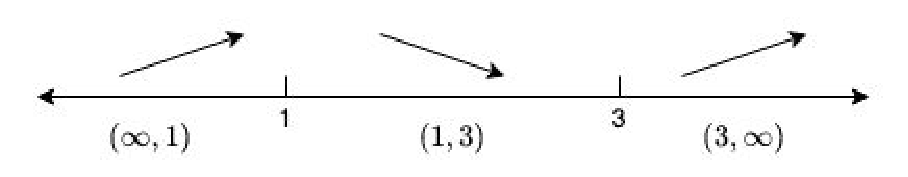
\includegraphics[width=0.5\textwidth]{Diagram_P15.eps}
%\caption{Problem 17(b) }
\end{figure}

\item For the function $f(x)=x^{4}-8x^{3}-72x^{2}+31x+111$, find the inflection points. Determine the intervals for which $f(x)$ is concave upwards and concave downward. 
    \subitem{1. Derivatives:} 
\begin{align*}
                   f^{\prime}(x)& = 4x^{3}-24x^{2}-144x+31\\
                  f^{\prime\prime}(x) & = 12x^{2}-48x-144
\end{align*}
  \subitem{2. Critical Number: } Set $f^{\prime\prime}(x)=0$ and solve for $x$.
\begin{align*}
             f^{\prime\prime}(x)& = 0\\
                12x^{2}-48x-144 & = 0\\
                   12(x-6)(x=2) & = 0\\
                    x=-2 & \text{ or } x=6
\end{align*}
   \subitem{3. Number Line} 
\begin{align*}
f^{\prime\prime}(-7)& = 12(-7)^{2}-48(-7)-144=780>0, \ \ \ \text{Concave Up}\\
 f^{\prime\prime}(0)& = 12(0)^{2}-48(0)-144=-144>0, \ \ \ \text{Concave Down}\\
 f^{\prime\prime}(3)& = 12(3)^{2}-48(3)-144=-180>0, \ \ \ \text{Concave Down}
\end{align*} 
\begin{figure}[H]
\centering
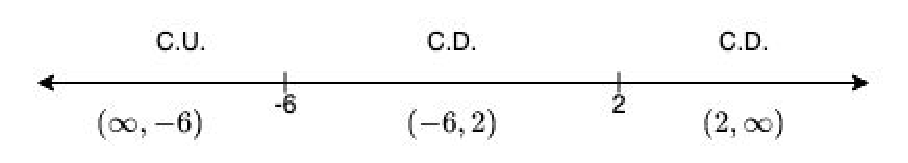
\includegraphics[width=0.5\textwidth]{Diagram_P16.eps}
%\caption{Problem 17(b) }
\end{figure}


%%%%%%%%%%%%%%%%%%%%%%%%%%%%%%%%%%%%%%%%%%%%%%%%%%%%%%%%-----New Page-----%%%%%%%%%%%%%%%%%%%%%%%%%%%%%%%%%%%%%%%%%%%
\newpage

\item Sketch the graph of $y = f(x)$, where $f(x) = x^{3} - 12x^{2} + 36x$ in the usual xy-plane.
\begin{enumerate}
  \item Find the domain, $x$-intercept and $y$-intercept of $f$.
    \subitem{1. Domain:} the function is polynomial, thus the domain is $(-\infty, \infty)$
    \subitem{2. x-intercept: } Set $f(x)=0$ and solve for $x$.
\begin{align*}
                   f(x)& = 0\\
 x^{3} - 12x^{2} + 36x & = 0\\
            x(x-6)^{2} & = 0\\
                     x=0 & \text{ or } x=6
\end{align*}
    \subitem{3. y-intercept: } Find $(0, f(0))$. that is $(0,0)$
  \item Calculate the derivative $f^{\prime}(x)$ and find the critical numbers of $f$. Make a number line and determine the intervals for which $f$ is increasing, decreasing.
  \subitem{1. Derivative:} $f^{\prime}(x)=3x^{2}-24x+36$
  \subitem{2. Critical Number: } Set $f^{\prime}(x)=0$ and solve for $x$.
\begin{align*}
                   f^{\prime}(x)& = 0\\
                  3x^{2}-24x+36 & = 0\\
            3(x-2)(x-6) & = 0\\
                     x=2 & \text{ or } x=6
\end{align*}
   \subitem{3. Number Line} 
\begin{align*}
 f^{\prime}(0)& = 3(0)^{2}-24(0)+36=36>0, \ \ \ \text{Increasing}\\
f^{\prime}(3)& = 3(3)^{2}-24(3)+36=-9<0, \ \ \ \text{decreasing}\\
f^{\prime}(7)& = 3(7)^{2}-24(7)+36=15>0, \ \ \  \text{Increasing}
\end{align*} 
\begin{figure}[H]
\centering
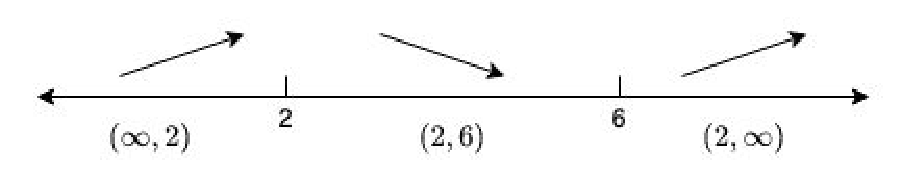
\includegraphics[width=0.5\textwidth]{Diagram_1.eps}
%\caption{Problem 17(b) }
\end{figure}
  \item Calculate the second derivative $f^{\prime\prime}(x)$ and find the possible inflection point of $f$. Make a number line and determine the intervals for which $f$ is concave up and concave down.
    \subitem{1. Derivative:} $f^{\prime}(x)=6x-24x$
  \subitem{2. Critical Number: } Set $f^{\prime}(x)=0$ and solve for $x$.
\begin{align*}
                   f^{\prime}(x)& = 0\\
                          6x-24 & = 0\\
                         6(x-4) & = 0\\
                               x&=4 
\end{align*}
   \subitem{3. Number Line} 
\begin{align*}
 f^{\prime\prime}(0)& = 6(0)-24=-24<0, \ \ \ \text{Concave Down}\\
 f^{\prime\prime}(7)& = 6(7)-24=18>0, \ \ \ \text{Concave Up}
\end{align*} 
\begin{figure}[H]
\centering
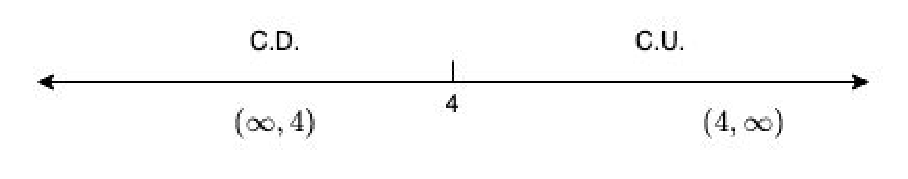
\includegraphics[width=0.5\textwidth]{Diagram_2.eps}
%\caption{Problem 17(b) }
\end{figure}
  \item  Use your information to determine the local extrema and the inflection points of $f$. Calculate the $y-values$ of each local extrema and inflection point.
  \subitem{1. Loacal maximum: } based on First Derivative Test and information in (b), Function arrive at local maximum at $x=6$. i.e. piint $(6, 0)$. 
  \subitem{2. Loacal minimum: } based on First Derivative Test and information in (b), Function arrive at local maximum at $x=2$. i.e. piint $(2, 32)$. 
  \subitem{3. Inflection Point: } based on Second Derivative and information in (c), Function have a inflection point at $x=4$. i.e. piint $(4, 16)$. 
  \item Use your information to sketch a graph of $f(x)$.
\begin{figure}[H]
\centering
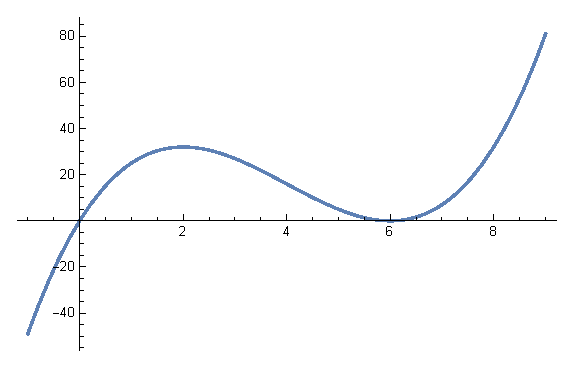
\includegraphics[width=0.3\textwidth]{Diagram_3.eps}
%\caption{Problem 17(b) }
\end{figure}
\end{enumerate}


%%%%%%%%%%%%%%%%%%%%%%%%%%%%%%%%%%%%%%%%%%%%%%%%%%%%%%%%-----New Page-----%%%%%%%%%%%%%%%%%%%%%%%%%%%%%%%%%%%%%%%%%%%
%\newpage
%
%\item We need to make a (right circular) cylindrical metal soup can with a closed top and bottom and with a volume of 175 cubic inches. Find the base radius and the height of such a cylinder that requires the least amount of metal.
%
%\vfill
%
%
%
%
%\item Which point on the graph of $y=4-x^{2}$ are closed to the point $(0, 2)$
%
%
%\vfill



\end{enumerate}
\end{document}

